\documentclass[tikz, border=5pt]{standalone}

% Adapted from:
% https://tex.stackexchange.com/a/26161/181375
% https://tex.stackexchange.com/a/305529/181375
\tikzstyle{venn circle}=[draw, circle, minimum width=6cm, fill=#1, fill opacity=0.4, text opacity=1]

% Colours from:
% https://nemo.kiwi/latex/colors.tex
\definecolor{red}{RGB}{175, 49, 39}
\definecolor{orange}{RGB}{217, 156, 55}
\definecolor{green}{RGB}{144, 169, 84}
\definecolor{grey}{rgb}{0.33, 0.41, 0.47}
\definecolor{blue}{rgb}{0.29, 0.59, 0.82}

\begin{document}
	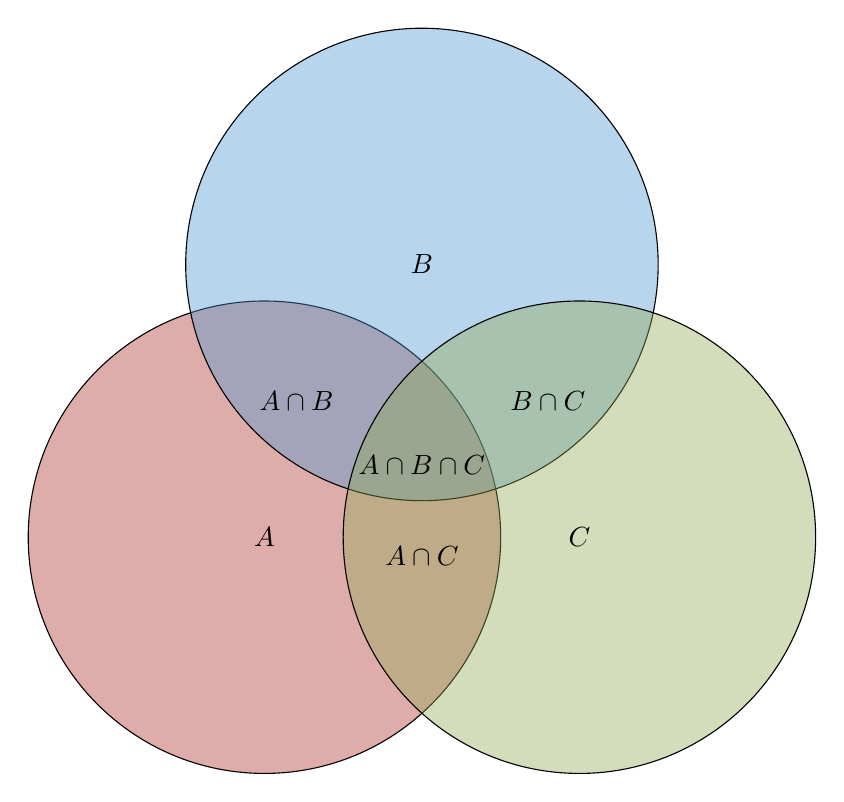
\begin{tikzpicture}
		\node [venn circle = red] (A) at (0,0) {$A$};
		\node [venn circle = blue] (B) at (60:4cm) {$B$};
		\node [venn circle = green] (C) at (0:4cm) {$C$};
		
		\node[left] at (barycentric cs:A=1/2,B=1/2) {$A \cap B$}; 
		\node[below] at (barycentric cs:A=1/2,C=1/2) {$A \cap C$};   
		\node[right] at (barycentric cs:B=1/2,C=1/2) {$B \cap C$};   
		\node[below] at (barycentric cs:A=1/3,B=1/3,C=1/3){$A \cap B \cap C$};	
	\end{tikzpicture}
\end{document}